
\documentclass[11pt]{article}
\usepackage[margin=1in]{geometry}
\usepackage{amsmath}
\usepackage{amsfonts}
\usepackage{graphicx}
\usepackage{booktabs}
\usepackage{float}
\usepackage{authblk}
\usepackage{hyperref}
\hypersetup{colorlinks=true, linkcolor=blue, citecolor=blue, urlcolor=blue}

% ----------------------------------------------------------------------
% Title
% ----------------------------------------------------------------------
\title{\vspace{-1em}Weighted Losses: The Grand Unified, Lottery-free, Cliff-free Anti-Tanking Solution}

\author{}
\date{}

\begin{document}

\maketitle
\thispagestyle{empty}
\vspace{-2em}

\textbf{Abstract:} Tanking is antithetical to the integrity of competition, but none of the existing solutions simultaneously align incentives while avoiding cliffs, situations where incentives change drastically game-to-game. Teams should draft in order of the most cumulative weighted losses, meaning losses are increasingly penalized as the season progresses for teams with poor records. 

For game number $n$ and win rate $w_{n}$, the weighted loss for a single game is 
\begin{equation}
  \ell(n, w_{n}) =
  \begin{cases}
    1 & n \le \underline{N}, \\[6pt]
    \displaystyle 1 - f(n)\,\Bigl(1 - \min(w_{n}/p,\,1)^{\gamma}\Bigr)
    & \underline{N} > n \le \overline{N}
  \end{cases}
\end{equation}
where the timing function is 
\begin{equation}
  f(n) = A \,(n - \underline{N})^{k}.
\end{equation}
The parameter $p$ is the win rate threshold below which teams incur a penalty. The game value $\overline{N}$ is the maximum number of games, 82 for the NBA, while $\underline{N}$ is the threshold game where the penalties begin. The parameters $\gamma, k, A$ are all positive.

For teams with winrate $w_{n}<p$, the weighted loss is decreasing in $n$ and increasing in $w_{n}$ so penalties increase as a team's performance declines and the season approaches the end.

The values for $(\underline{N}, A)$ are set to (40, 0.25) so the initial penalty halfway through the season is modest compared to an unweighted loss of one. The other parameter values are chosen according to the following conditions, where $cw\ell(n,\,w)$ is cumulative weighted losses up to game $n$ for a team with a constant win rate.
\begin{align}
  \ell(\overline{N}, 0) &= -1\label{eq:c2}\\
  \ell(\overline{N},\,0.4) &= 0 \label{eq:c3}\\
  cw\ell(\overline{N},\,0.2) &= cw\ell(\overline{N},\,0.4) \label{eq:c4}
\end{align}
The first condition means a team with no wins in a season receives a weighted loss of -1 for the last game, reflecting a significant penalty. The second condition ensures that a team on the edge of playoff contention with a win rate of 0.4 has a weighted loss of zero so there is no incentive regarding draft position.

The last condition is inspired by the new NBA plan where the fourth and tenth worst teams have the same odds of getting the top draft pick, though the weighted loss system has no cliff. (With the new NBA system, the chance of the top pick for a team jumps from 5.4\% to 8.1\% if it moves from eleventh worst to tenth.) Given these three conditions, the weighted loss parameters are $(\gamma,k,p)=(0.9898, 0.5563, 0.8058)$.

\begin{figure}[h]
  \centering
  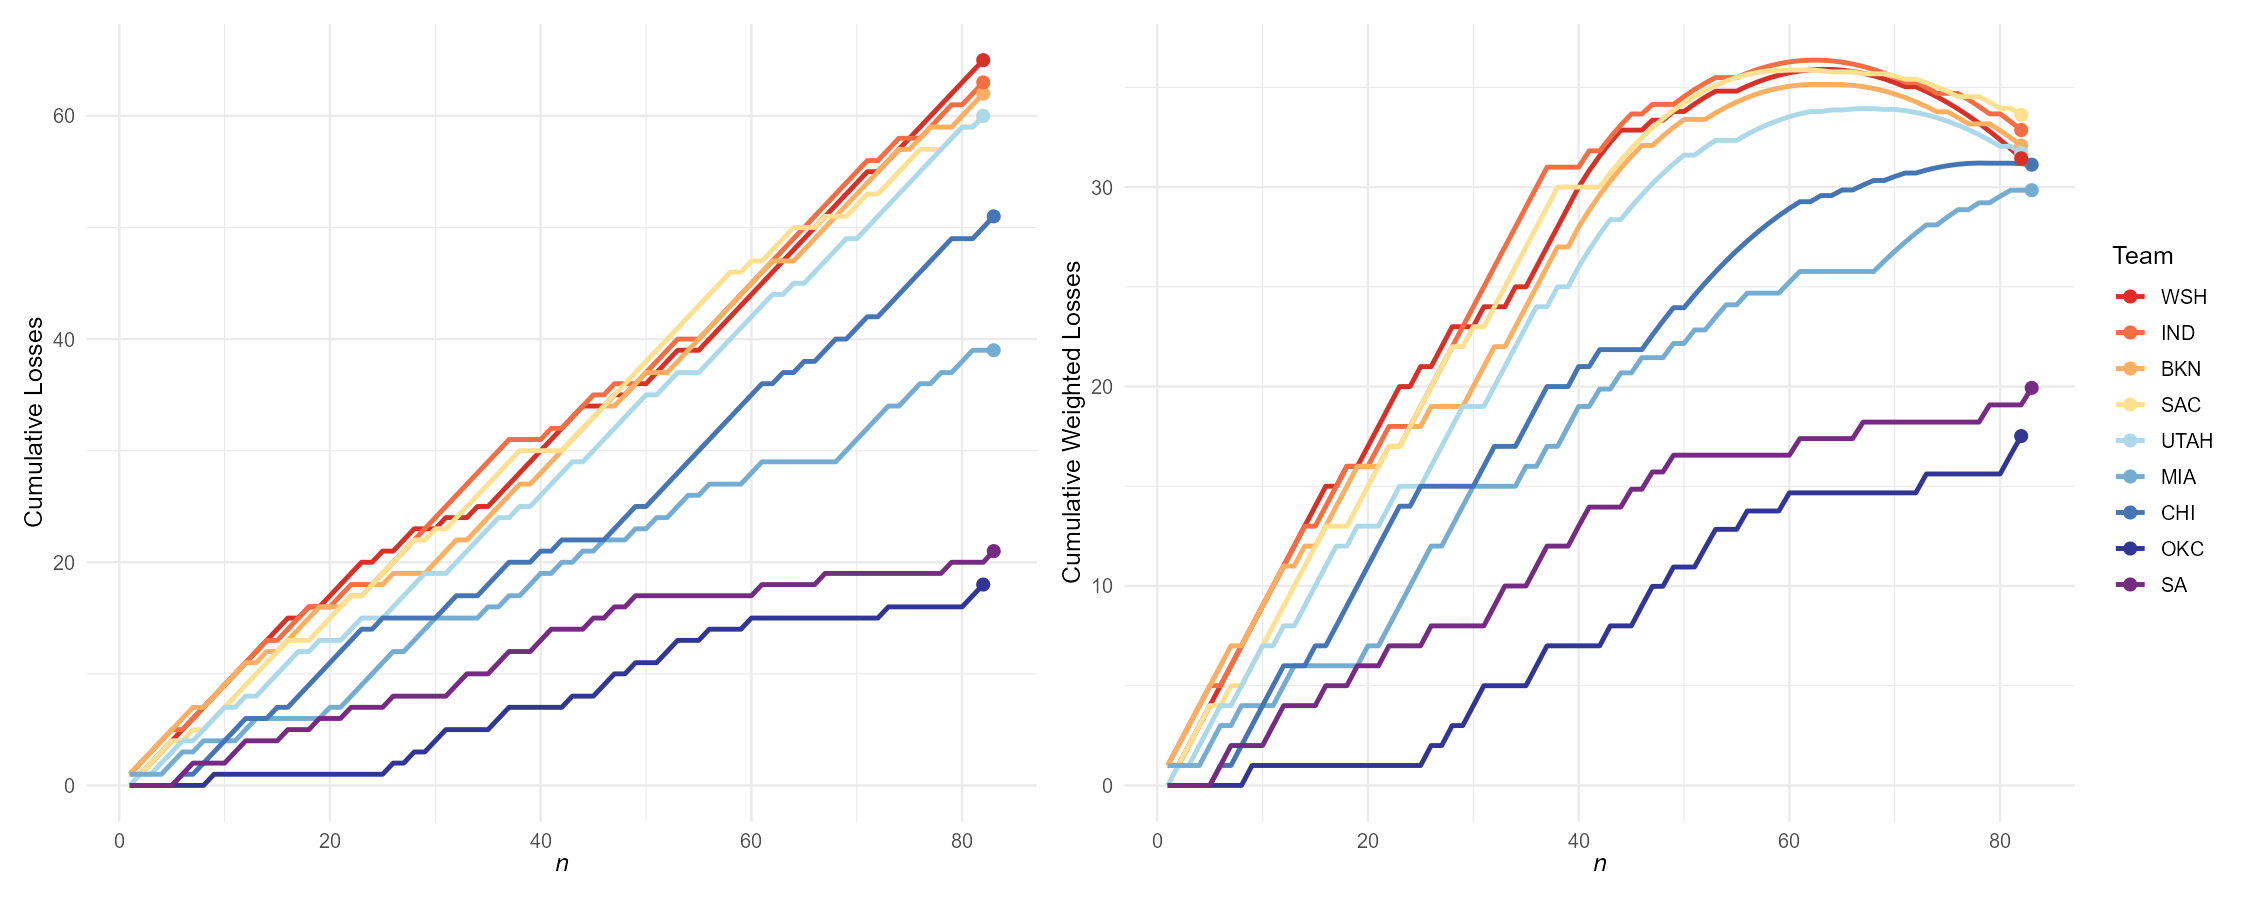
\includegraphics[width=0.9\textwidth]{graphics/tanking_lines_2panel_selectteams.png}
 \end{figure}

The figure shows the evolution of the unweighted and weighted losses for the 2025-2026 NBA season for the five worst teams, the two best teams and the two 10 seeds, Miami and Chicago, the teams with the final play-in seed. By design, the teams with the most losses are most affected by the weighting, and the effect increases as the season progresses. With weighted losses, incentives would change, so the second panel is not a prediction. The best teams are almost unaffected. The cumulative weighted loss curve for the 10 seeds is flat, reflecting the last condition.

The table shows the new draft order, sorted by weighted rank, with $\Delta$Rank giving the change from each team's unweighted-loss rank. Again, tanking teams are penalized, but the order is not drastically altered.

The weighted loss formula obviates the need for a lottery and removes most of the incentive to tank while maintaining a system where weaker teams draft before the stronger. The parameter values can accommodate a range of preferences.

\bigskip

\begin{table}[H]
\centering
\begin{minipage}[t]{0.48\textwidth}
\centering
\begin{tabular}{lrrr}
\toprule
Team & Losses & Wt.\ Losses & $\Delta$Rank \\
\midrule
NO   & 56 & 35.8 & +6 \\
SAC  & 60 & 34.1 & +2 \\
IND  & 63 & 33.4 & $-$1 \\
BKN  & 62 & 32.6 & $-$1 \\
MIL  & 50 & 32.4 & +5 \\
UTAH & 60 & 32.2 & $-$2 \\
DAL  & 56 & 32.1 & 0 \\
WSH  & 65 & 32.0 & $-$7 \\
CHA  & 38 & 31.8 & +6 \\
MEM  & 57 & 31.3 & $-$4 \\
CHI  & 51 & 31.3 & $-$2 \\
LAC  & 40 & 31.1 & 0 \\
GS   & 45 & 30.7 & $-$2 \\
POR  & 40 & 30.6 & $-$2 \\
MIA  & 39 & 29.8 & $-$1 \\
\bottomrule
\end{tabular}
\end{minipage}%
\hfill
\begin{minipage}[t]{0.48\textwidth}
\centering
\begin{tabular}{lrrr}
\toprule
Team & Losses & Wt.\ Losses & $\Delta$Rank \\
\midrule
ATL  & 36 & 29.6 & +3 \\
ORL  & 37 & 29.1 & $-$1 \\
PHI  & 37 & 28.9 & $-$2 \\
PHX  & 37 & 28.5 & $-$3 \\
TOR  & 36 & 28.3 & $-$1 \\
MIN  & 33 & 26.9 & 0 \\
CLE  & 30 & 26.1 & 0 \\
HOU  & 30 & 25.4 & $-$1 \\
LAL  & 29 & 25.1 & 0 \\
NY   & 29 & 25.0 & $-$1 \\
DEN  & 28 & 24.1 & 0 \\
BOS  & 26 & 23.3 & 0 \\
DET  & 22 & 20.3 & 0 \\
SA   & 21 & 19.8 & 0 \\
OKC  & 18 & 17.3 & 0 \\
\bottomrule
\end{tabular}
\end{minipage}
\end{table}

\end{document}
